\section{Introduction}
In this chapter we are going to present some of the recent work and research that was done regarding skin cancer detection and classification using machine learning , we are going to explore the various methods, tools, new ideas and challenges that was handeled by researchers for the hope of getting a clear understanding of the problem and how to go about solving it depending on each one's conditions, requirements and goals.



\section{skin cancer detection and classification using machine learning}
\begin{description}
    \item [proposed methodology]
    the proposed methodology in this article ~\cite{Krishna2020} uses a 6 step process (input data - preprocessing - segmentation - feature extraction - classification - output data)
    \item [input data] 
        dermoscopic images from the ISIC ( International Skin Imaging Collaboration) 2019 challenge containing 8 classes of skin cancer, and for simplisity reasons only 800 images out of 25000 is used.
    
    \item [preprocessing]
        because of the heteroginity of the input data a preprocessing step is required to inhance the quality of images and remove irrelevant parts. the main technices used here are gray scale conversion and the application of the Gaussian and median filter for noise removal and enhancement, and for the unwanted hair they applied the Dull Razor method (a preprocessing algorithm), as shown in figure ~\ref{fig:Preprocessing}

    \item [segmentation]
        segmnetation is used to extract the region of interest and for that they used a k-means clustering algorithm as shown in figure \ref{fig:segmentation}
        
    \item [feature extraction]
        for this they used 2 well know methods, ABCD method and GLCM. ABCD is used in dermatological applications and diagnosis for skin lesions such as melanomas and it is the abreviation of Asymmetry, Border, Color and Diameter. Grey Level Co-occurrence Matrix (GLCM) is used for texture analysis, other features are also used in addition to these 2 methods for further classification such as Autocorrelation, correlation, Standard vector...etc
    
    \item [classification]
        for classification they used MSVM (Multi-class Support vector machine) machine learning algorithm, they used trainning and testing ratios of 70:30 and obtained an acuuracy of 96.25\% and the confusion matrix shown in figure \ref{fig:confusion-matrix}
\end{description}

\begin{figure}[htbp]
\begin{center}
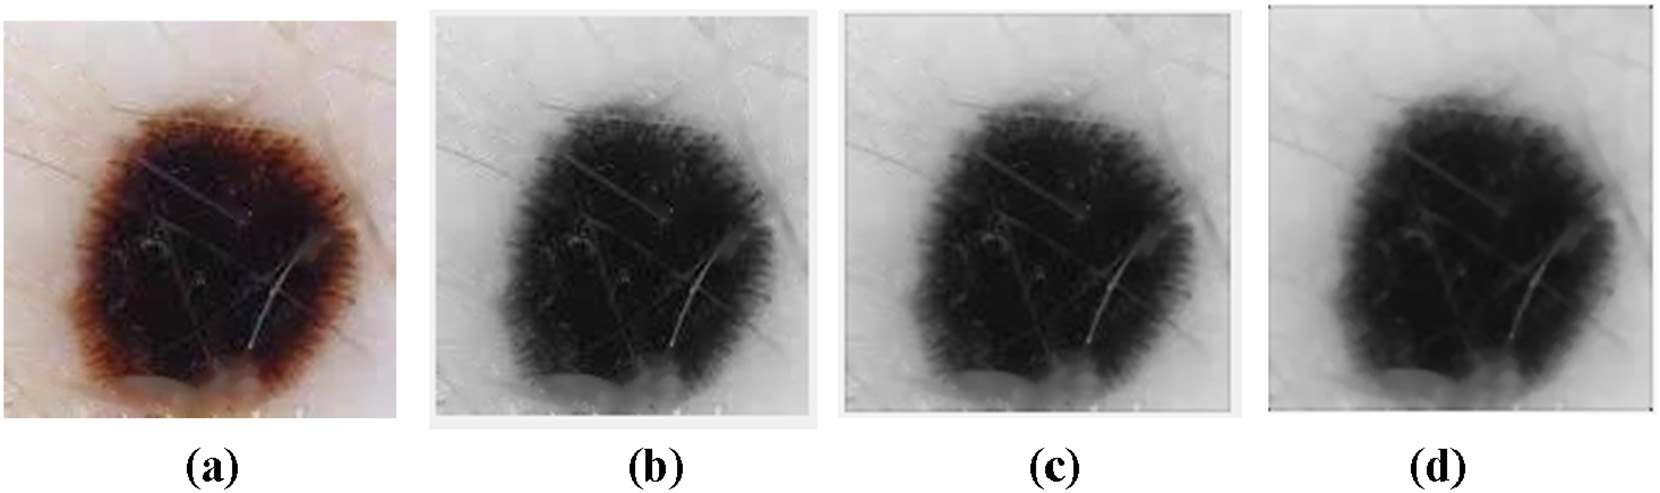
\includegraphics[width=15cm]{./chapter-03-state-of-the-art/preprocessing.png}
\end{center}
\caption{Preprocessing: (a)Dull razor image, (b) Gray scale image, (c) Gaussian filter, (d) Median filter.}
\label{fig:Preprocessing}
\end{figure}




\begin{figure}[htbp]
\begin{center}
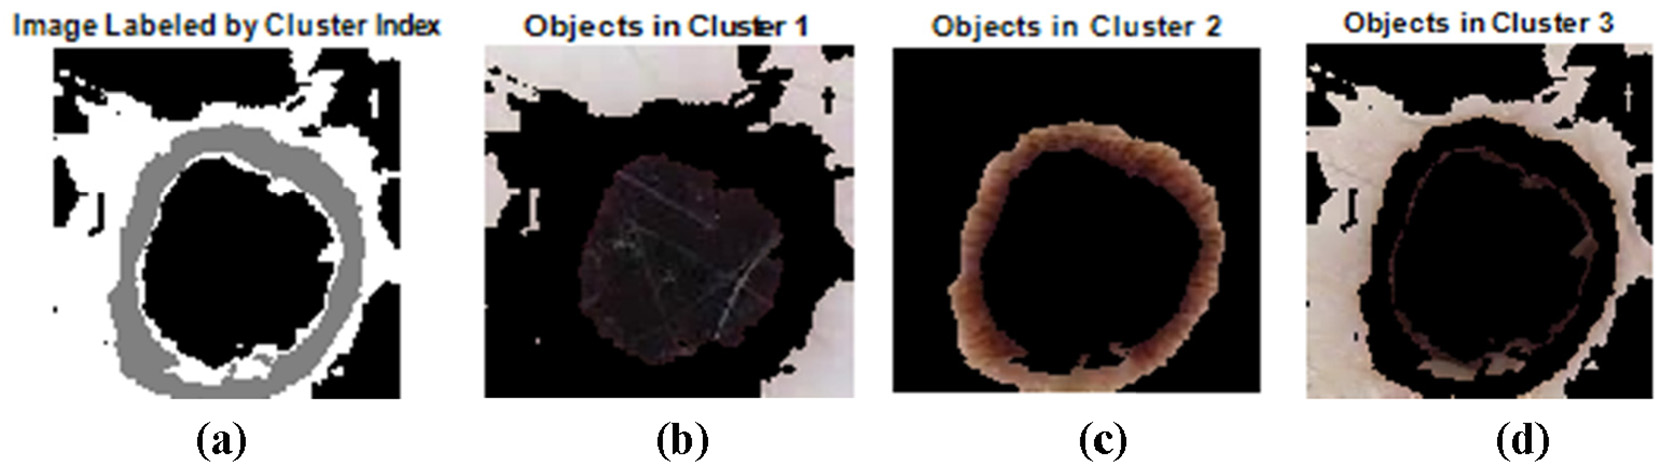
\includegraphics[width=15cm]{./chapter-03-state-of-the-art/segmentation.png}
\end{center}
\caption{Segmentation: (a) Image labelled by cluster index, (b) Objects in cluster 1, (c) Objects in cluster 2, (d) Objects in cluster 3.}
\label{fig:segmentation}
\end{figure}


\begin{figure}[htbp]
\begin{center}
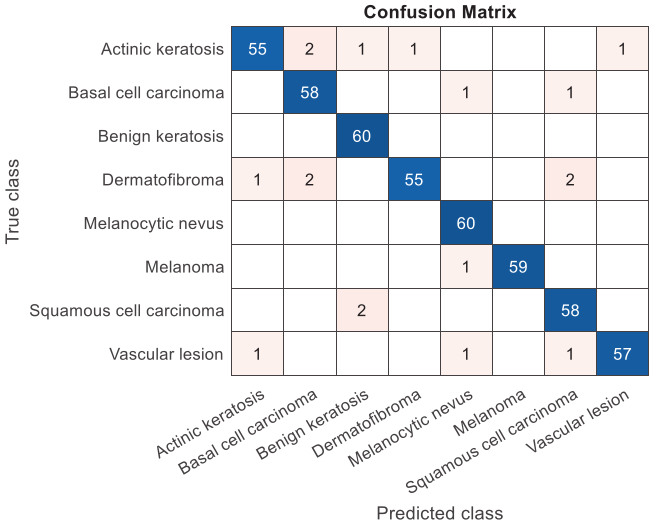
\includegraphics[width=15cm]{./chapter-03-state-of-the-art/confusion-matrix.png}
\end{center}
\caption{Confusion Matrix}
\label{fig:confusion-matrix}
\end{figure}



%=================================================================

\section{Finding reduced Raman spectroscopy fingerprint of skin samples for melanoma diagnosis through machine learning}
    This article ~\cite{Daniella2021} uses a new non invasive approach to classify malignant and benign tumors, and that is by using Raman spectral data instead of images, Raman Spectroscopy is a way to analyse the chemical structure using light and vibrational energy modes of molecules ~\cite{Edinburgh}
\begin{description}
\item[data and method] \hfill \\
    
    \textbf{dataset: }
    for the dataset they brought 33 benign and 51 malignant smaples and cut them into regular cuts of $2mm^3$, a layser was used to excite the samples to collect the Raman signals using special tools after this they aquired 436 Raman spectra. and they focused on the biological fingerprint spectral region from 800 to 1800 $cm^-1$

    \textbf{Fluorescence background data pre-process: }
    Fluorescence is a radiation that is emitted by molecules after interacting with electromagnetic radiation and this could overshdow and disturb the study of Raman spectra, to deal with this noise they used a low frequency laser to lower the probability of fluorescence emissions and by this they could jump the preprocessing step.
\item[feature extraction]
    they divided the obtained spectrums into subsequences (local spectrums) and extracted some statistical measures from it such as arithmetic mean, standard deviation, derivative ...etc

\item[results and discussion]
    these statistical features were then given to a machine learning classification algorithm, a complex dicision tree impimented using lightGBM (open source software), other algorithms were also used such as K-nearest neighbors and XGBOOST (Extreme Gradient Boosting an open source software) but the best performance was obtained using lightGBM.
    further research led them to only use the derivative as a feature and a spectral region from 896 to 1039 $cm^-1$ because these two were proved the most discriminative information between malignant and benign tumors and by this they obtained a high performant model ($AUC \geq 0.97$) shown in figure \ref{fig:roc}
\end{description}

\begin{figure}[htbp]
\begin{center}
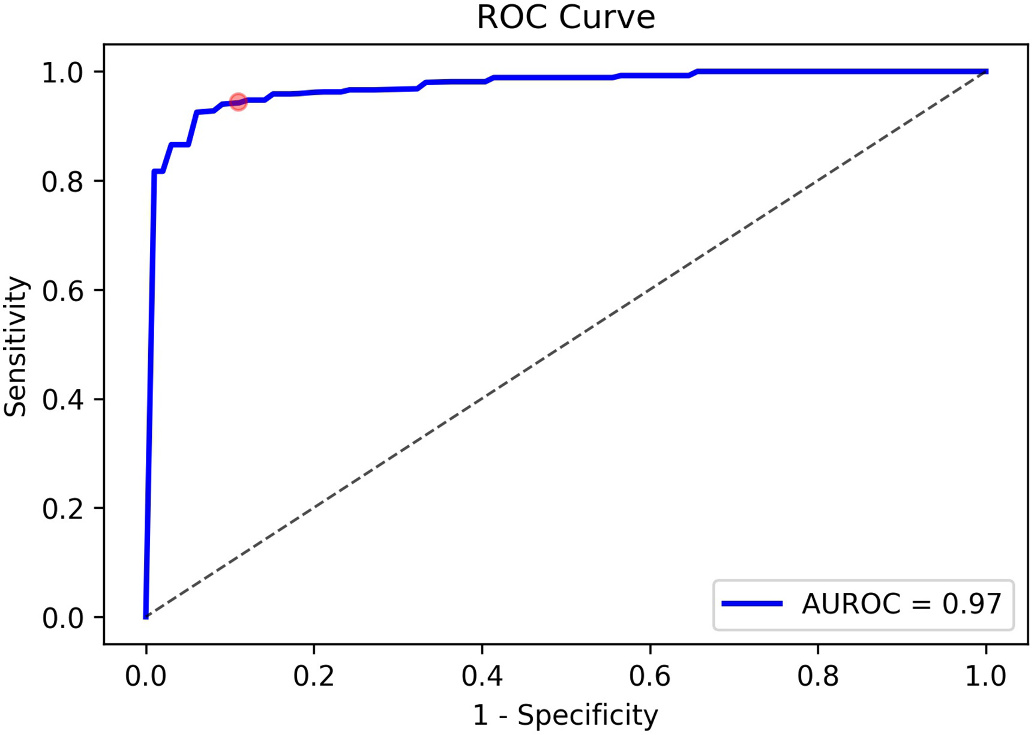
\includegraphics[width=10cm]{./chapter-03-state-of-the-art/ROC.png}
\end{center}
\caption{ROC}
\label{fig:roc}
\end{figure}






%================================================================

\section{Skin cancer detection: Applying a deep learning based model driven architecture in the cloud for classifying dermal cell images}
\begin{description}
\item[Summary] \hfill \\
in this paper ~\cite{Kadampur2020} the researchers are presenting a model driven approach to develop deep learning algorithms for detecting skin cancer by using a tool called DLS (deep learning studio) which is a software that allows you to build deep learning algorithms without being a specialist in programming languages, it presents a simple drag and drop interface for building models it also commes with desktop / cloud versions and community / enterprise editions with multi-GPU trainning and the possibility to obtain the code of the model, download the model and host it as a REST API (Representational state transfer Application programming interface), the interface dashboard is shown in figure ~\ref{fig:dls}
\item[Advantage] \hfill \\
the advantage of this non programatic approach is for researchers and practitionners to be able to create and test there own models without the need for prior programming knowledge
\item[Application and Results] \hfill \\
and then they procede using this tool DLS to show its efficacy and ease of use, they have built and tested 5 models using famous architectures squeeznet, densenet, and inception v3
with model1 aquiring an AUC of 99.77\% 
\end{description}


\begin{figure}[htbp]
\begin{center}
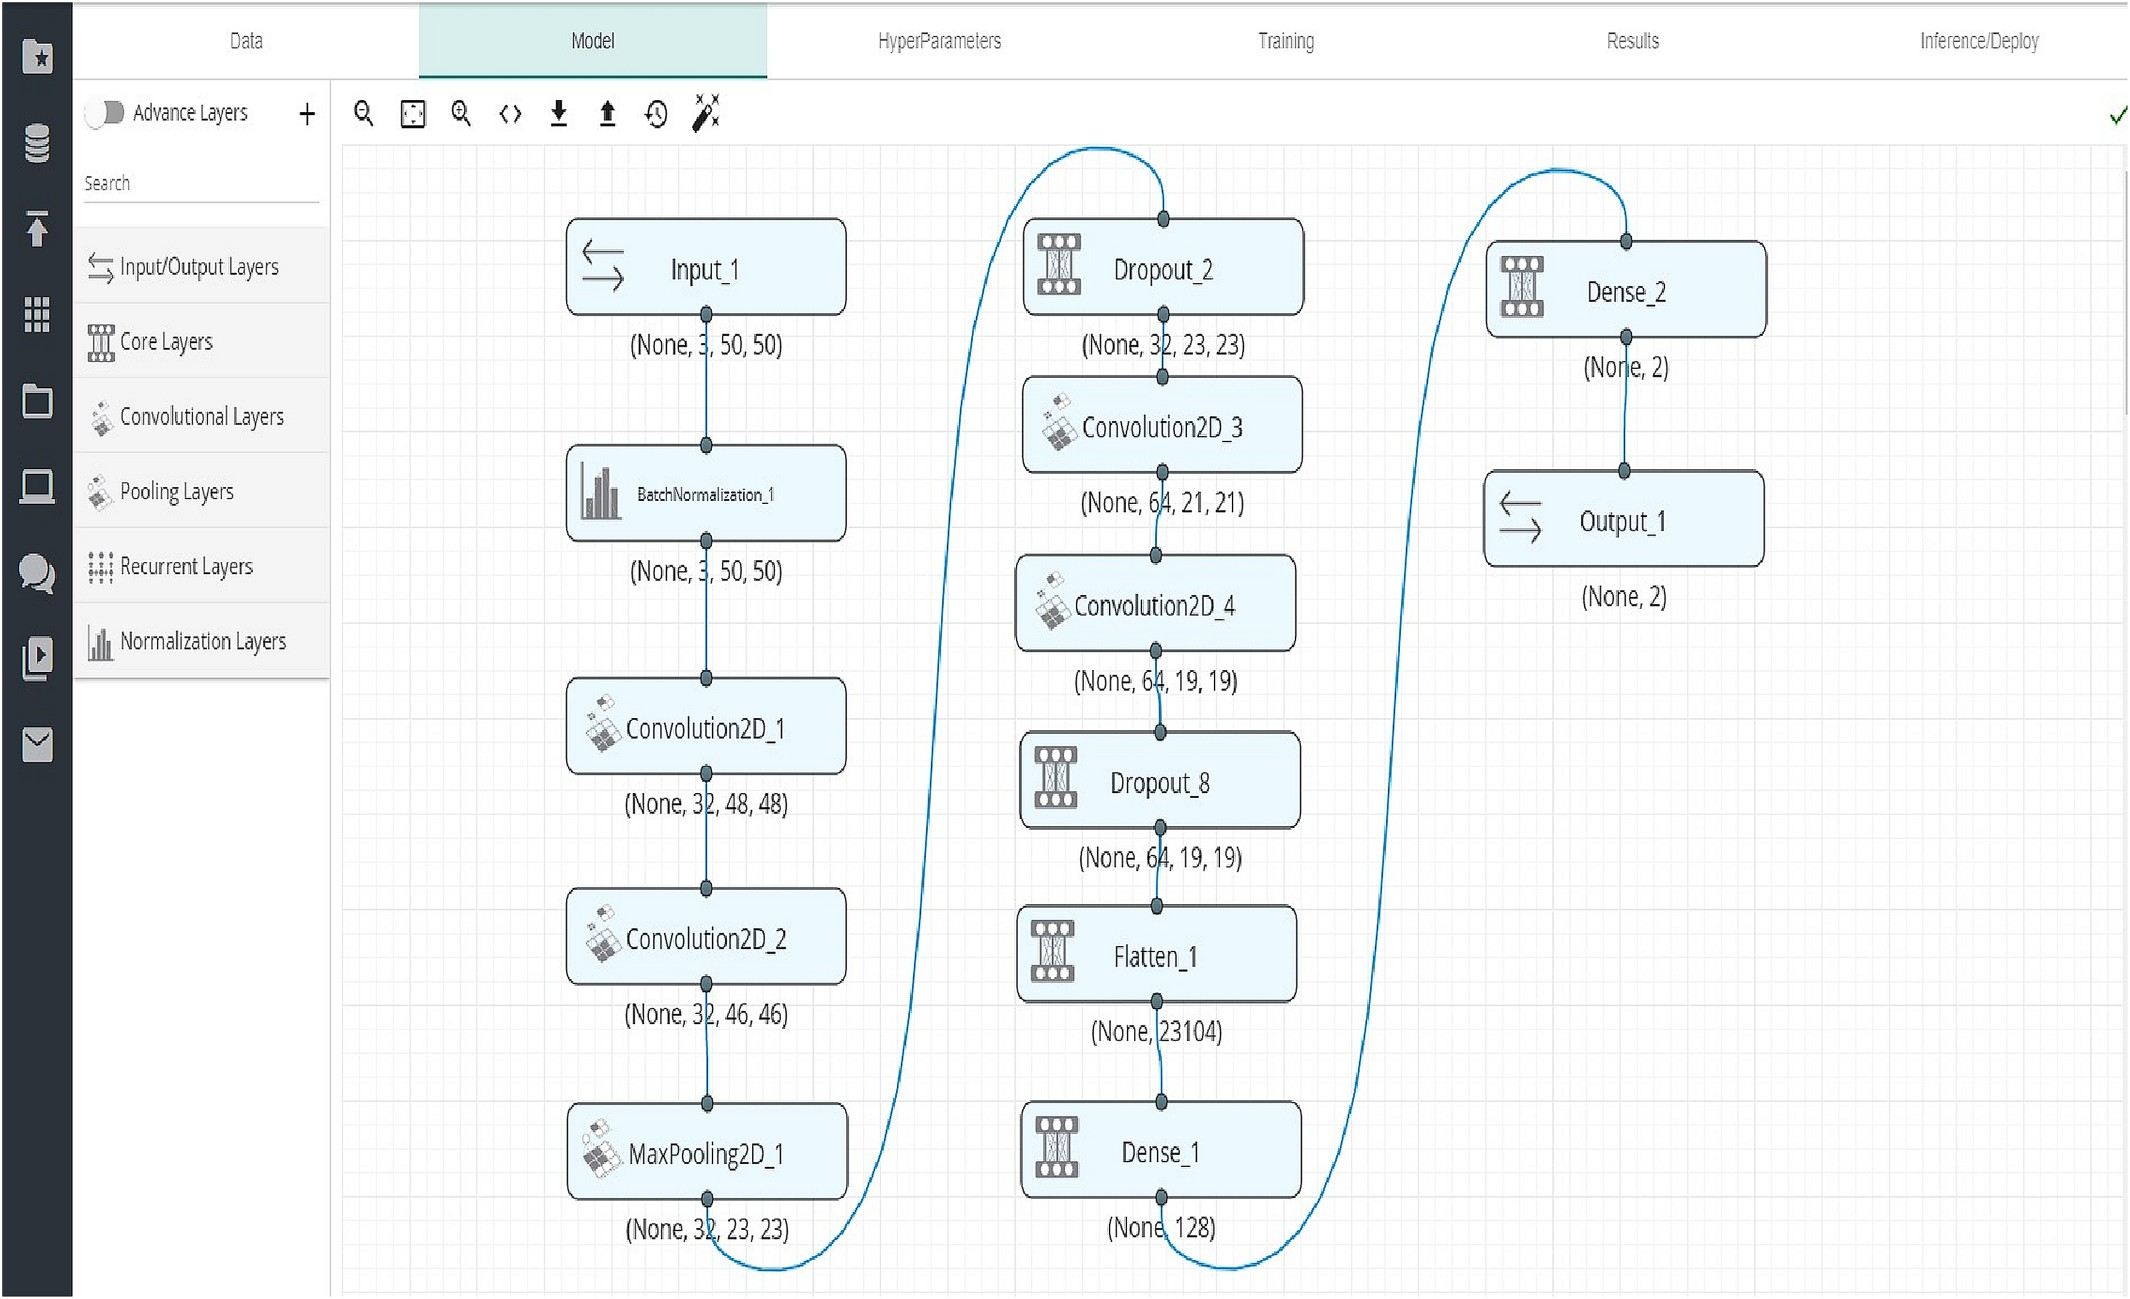
\includegraphics[width=12cm]{./chapter-03-state-of-the-art/dls.png}
\end{center}
\caption{DLS Interface}
\label{fig:dls}
\end{figure}



%========================================================================================


\section{The impact of patient clinical information on automated skin cancer detection}
In this work ~\cite{Pacheco2020} the researchers propose a new idea, which is the use  of clinical information in addition to the image dataset and the study of this addition's effect on the deep learning model's performance

\begin{description}
\item[dataset] \hfill \\
to build their hybrid dataset, they proposed a mobile application given to doctors and students to help collect the necessary data from Dermatological Assistance Program (PAD) dataset at the Federal University of Espírito Santo (UFES), which consists of images of the lesion, their clinical diagnosis and 8 clinical information based on common questions that dermotologists ask:
\begin{itemize}
    \item age
    \item part of the body where the lesion is located,
    \item if the lesion itches,
    \item bleeds or has bled,
    \item hurts, 
    \item has recently increased, 
    \item has changed its pattern, 
    \item and if it has an elevation
\end{itemize}

a total of 1612 images of 6 lesions

because the image dataset is imbalanced they used multiple strategies to overcome that such as, transfer learning (refining a pretrained model on there dataset) , data augmentation, horizontal and vertical rotations, adjusting brightness...etc, and for the clinical data they used one-hot encoding (converting categorical data to augment the performance) which transformed the 8 features collected to an array of 28 values 

\item[trainning] \hfill \\
    they used 4 CNN architectures VGGNet-13/19-bn, ResNet-50/101, MobileNet, GoogleNet
    now a problem arised when trying to combine (by concatenation) clinical data with image features extracted by the CNN feature extractor because image features are far more great in size then clinical data, this imbalance is not good for the trainning and classification because the effect of image features will be greater then the clinical data, that is why they  they implimented an NN feature reducer on the extracted image features before combining it with the clinical data as shown in figure ~\ref{fig:model} [clinical-image.png] and the classifier is another neural network that assigns the probabilities for each skin lesion

\item[testing the effect of adding clinical data] \hfill \\
    they executed 2 scenarios for that, 1 using models trained only with images, 2 using models trained with images + clinical data then they calculated multiple  performance metrics accuracy , balanced accuracy , weighted precision , weighted recall , weighted F1 score  and area under the curve and they found almost all models was improved by 7\% in almost all metrics and the best model ResNet-50 presented an $AUC \geq 95.8\%$ 

\item[conclusion] \hfill \\
    clinical information does make a difference when trainning ML models to classify skin cancer 
\end{description}



\begin{figure}[htbp]
\begin{center}
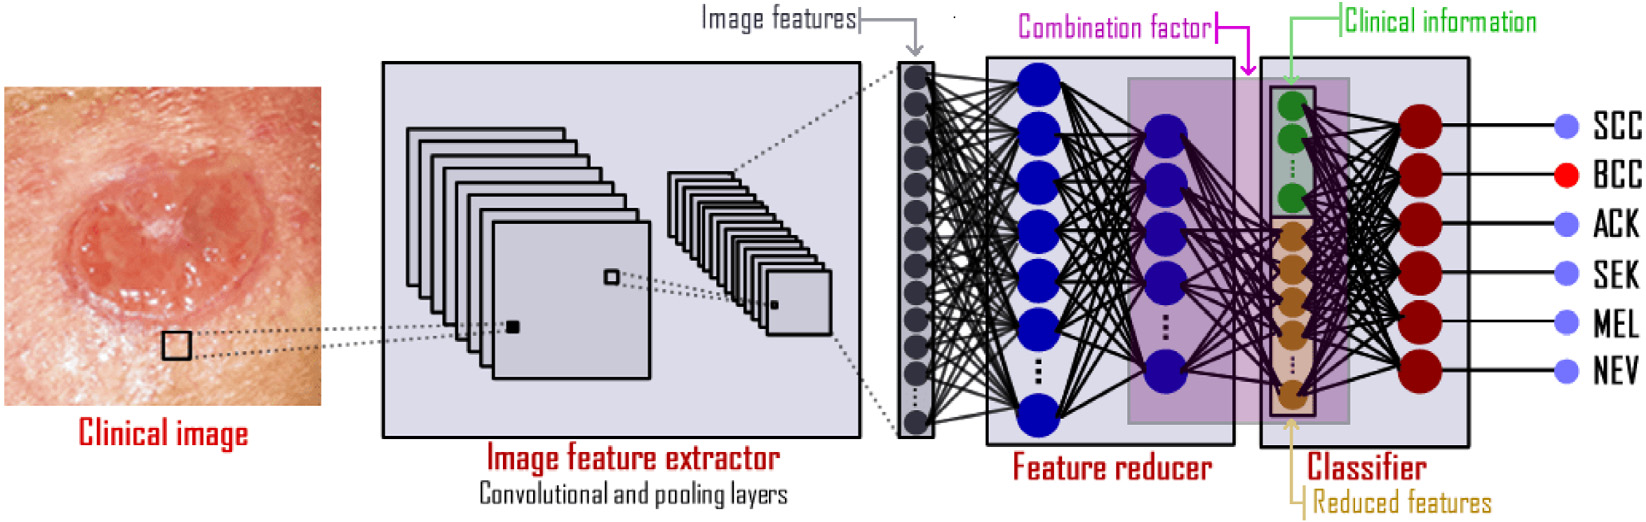
\includegraphics[width=15cm]{./chapter-03-state-of-the-art/clinical-image.png}
\end{center}
\caption{Model}
\label{fig:model}
\end{figure}


% \begin{figure}[htbp]
% \begin{center}
% 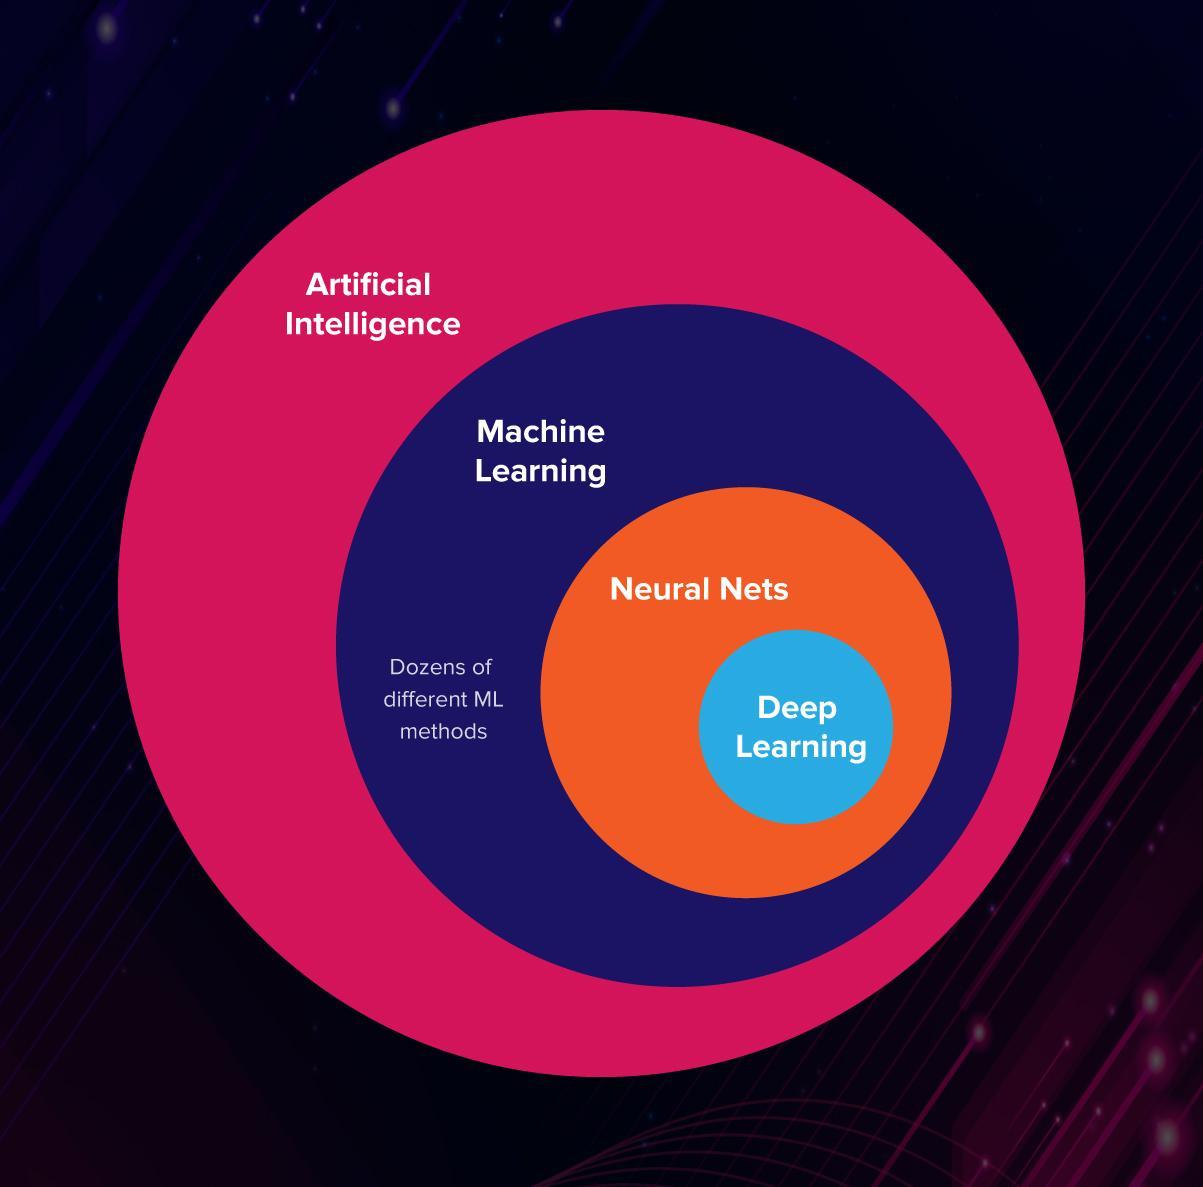
\includegraphics[width=2cm]{./chapter-03-state-of-the-art/versus.jpg}
% \end{center}
% \caption{}
% \label{fig:}
% \end{figure}
